%EXP

\subsection{Experimental Setup}

Each read was assembled with SOAPdenovo2, with the k-mer length set to 51, reads cut off after 100 base pairs (original length of 180 base pairs), and the average insert size set to 350 in accordance with the reported average insert size reported in the MGWAS study \cite{qin041012}. Assembly for each file took 7-30 minutes, depending on the file size. The assembly of the patient files is embarrassingly parallel, so the assembly of each file could be done at the same time. Combining the files into one file took 2 minutes and 35 seconds. Assembly was used for all of the classification methods tested, because the combining of individual reads and reduction in total data size made classification feasible.

\subsection{Methods Tested}

This section provides an overview of the different methods that we compared our pipeline to. Our pipeline uses clustering, whereas the other methods do not. Instead, those methods directly compare individual reads instead of clusters. In order to do this, sequence reads were represented as counts of k-mers. k-mers are nucleotide strings of 
length k. Since there are four possible nucleotides, the number
of possible k-mers are \(4^k\). 
%For instance, if k=3, there are \(4^3\) = 64 possible k-mers, which are AAA, AAC, AAG, AAT, ACA, ACC, ..., TTT. 
%For a string "ATACGATA", the count for the k-mers is 2 for ATA, 1 for TAC, ACG, CGA, and GAT, and 0 for everything else. 
We wrote a script to represent the reads/contigs as vectors representing the k-mer counts in the string, and these feature 
vectors were used by the other methods. We tested possible k values 
from 1 to 6; since the number of possible k-mers is 
exponential in k, higher values for k quickly become impractical in both run time and memory usage. From experimental validation, we found a k-mer value of 3 to be the most effective. Converting the reads from their original string form to k-mer vectors with k=3 took 24 hours, 8 minutes, and 49 seconds.

%%%%%%%%%%%%%%%%%%%%%%%%%%%%%%%%

\subsubsection{CAMIL - Our Pipeline}

We implemented two different versions of the pipeline: one that uses D-BoW feature extraction, and one that uses H-BoW feature extraction. These results are denoted as ``CAMIL D-BoW" and ``CAMIL H-BoW", respectively, in the results tables and graphs. Clustering for the pipeline with UCLUST took 10 hours and 51 minutes. Without the assembly step reducing the size of the data, clustering would not have been feasible. Feature extraction and SVM-light classification took 10 minutes and 17 seconds to run for D-BoW, versus 5 minutes and 14 seconds for H-BoW.

\subsubsection{MISVM and sbMIL}

MISVM \cite{andrews02} and sbMIL \cite{bunescu07} are two of the classic Multiple Instance Learning algorithms that fall into what Amores calls the ``Instance Space" (IS) methods, in that they only use ``local" information based on comparisons between individual instances and treat bag labels as aggregations of instance labels \cite{amores13}. Additionally, both of these methods follow the standard MIL assumption that bags with negative labels contain only negative instances, whereas positive bags contain one or more positive instances \cite{amores13}. sbMIL specifically assumes that positive bags contain few positive instances \cite{bunescu07}. We include these algorithms as an example of many of the early MIL algorithms, which usually fell into the IS paradigm and used the standard MIL assumption. For the implementation of these methods, we used an open-source Python implementation by Doran \cite{doran14}, which is available on GitHub\footnote{https://github.com/garydoranjr/misvm}.

\subsubsection{GICF}

The Group-Instance Cost Function (GICF) is a method proposed by Kotzias et al. that learns instance labels in addition to group labels \cite{kotzias15}. The cost function uses a kernel that measures similarity between instances and a penalty on the difference between instance labels to generate instance labels \cite{kotzias15}. It then sets the group label to be the average instance label of all instances in that group, using a penalty on the difference between the predicted group label and the actual group label \cite{kotzias15}. Ideally, this would cause instances that are similar to each other to have similar predicted labels, and predicted group labels to correspond closely to reality. Unlike MISVM and sbMIL, GICF explicitly does not hold the standard MIL assumption, instead favoring the collective assumption. However, because this method compares only individual instances and not entire bags, and treats bag labels simply as aggregations of instance labels, GICF is still an Instance Space method.

\subsubsection{Original MGWAS Paper}

The methods in the original paper are neither MIL-based, nor are they entirely de novo apart from patient labels. The authors first performed de novo assembly with SOAPdenovo2 \cite{luo12} and then use a tool called MetaGeneMark \cite{zhu10, besemer99} for de novo prediction of genes from the assembled contigs \cite{qin041012}. They then combined these genes with an existing gene catalog, MetaHIT \cite{qin030410}, and carried out taxonomic assignment and functional annotation of the genes using the KEGG \cite{kanehisa00} and eggNOG \cite{powell12} databases, as well as 2,890 other reference genomes \cite{qin041012}. The authors defined gene markers by mapping the sequence reads from the MGWAS dataset to the updated gene catalog. They identified the 50 most important gene markers with the minimum redundancy - maximum relevance (mRMR) \cite{peng05} method, using the ``sideChannelAttack" R package and then used these 50 gene markers for SVM classification of T2D phenotype, using the ``e1071" R package for the SVM \cite{qin041012}. Thus, the method in the original paper first applies de novo assembly and gene prediction methods, but then uses a number of references to identify the gene markers to be used in classification. From their results, the authors generated an Area Under Curve - Receiver Operating Characteristic (AUC-ROC) graph. The authors did not provide a learned decision boundary in their supplementary tables, only the predicted values for each patient, so we manually computed the accuracy and F1 score with an optimally-chosen decision boundary. 

%%%%%%%%%%%%%%%%%%%%%%%%%%%%%%%%


\subsection{Results For Bag/Patient Labels}

\begin{table*}[t]
\begin{center} 
%\hfill
\begin{minipage}{0.4\textwidth}
\caption{Performance with even train/test split.} 
\label{tab:even-comp}
\begin{tabular}{|c|ccc|}\hline
Method & Accuracy & F1-Score & AUC-ROC\\\hline
MISVM & --- & --- & ---\\\hline
sbMIL & --- & --- & ---\\\hline
GICF & 63.04 & 68.33 & 66.19\\\hline %59.24,63.05,66.19
CAMIL D-BoW & 86.34 & 87.18 & 95.93\\\hline
CAMIL H-BoW & \bf{90.71} & \bf{89.70} & \bf{97.63}\\\hline
\end{tabular}
\end{minipage}
\bigskip
\begin{minipage}{0.4\textwidth}
\caption{Classification time with even train/test split.} 
\label{tab:time-comp}
\begin{tabular}{|c|c|}\hline
Method & Classification Time\\\hline
MISVM & ---\\\hline
sbMIL & ---\\\hline
GICF & 8 hours, 44 minutes, 27 seconds\\\hline
CAMIL D-BoW & \bf{6 minutes, 58 seconds}\\\hline
CAMIL H-BoW & 7 minutes, 56 seconds\\\hline
\end{tabular}
\end{minipage}
\begin{minipage}{0.4\textwidth}
\caption{Performance on subset of instances.}
\label{tab:train-comp}
\begin{tabular}{|c|ccc|}\hline
Method & Accuracy & F1-Score & AUC-ROC\\\hline
MISVM & 50.8 & ? & ?\\\hline
sbMIL & 50.8 & ? & ?\\\hline
GICF & ? & ? & ?\\\hline
CAMIL D-BoW & 90.70 & 90.91 & 97.45\\\hline
CAMIL H-BoW & \bf{94.19} & \bf{93.87} & \bf{97.87}\\\hline
\end{tabular}
\end{minipage}
\begin{minipage}{0.4\textwidth}
\caption{Performance with 23 patient test set.} 
\label{tab:test-comp}
\begin{tabular}{|c|ccc|}\hline
Method & Accuracy & F1-Score & AUC-ROC\\\hline
MISVM & --- & --- & ---\\\hline
sbMIL & --- & --- & ---\\\hline
GICF & 73.91 & 75.00 & 78.03\\\hline
mRMR + SVM & 82.61 & 82.76 & 87.12\\\hline 
CAMIL D-BoW & 91.30 & 92.31 & \bf{100.00}\\\hline
CAMIL H-BoW & \bf{100.00} & \bf{100.00} & \bf{100.00}\\\hline
\end{tabular}
\end{minipage}
\end{center}
\end{table*}

%\begin{table}[t]
%\begin{center}

%\end{center}
%\end{table}

%\begin{table}[t]
%\begin{center}

%\end{center}
%\end{table}

In the original MGWAS paper, the authors use 344 patients as a training set and 23 as a test set. However, in their reported AUC-ROC reflects the performance of of the mRMR + SVM approach on the 344 patients whose data was used to generate the gene markers that were used for classification. Essentially, they tested the performance of their approach on the training data. We thus applied our CAMIL pipeline in the same manner, using the same 344 patients as both the training and test set. The results are shown in Table \ref{tab:train-comp}, which demonstrates that both CAMIL variants significantly outperformed the mRMR + SVM approach in all metrics by about 14-17\%, with the CAMIL H-BoW version performing the best. Since this is not a typical way of assessing classification performance, we ran several other experiments, discussed below. 

The MGWAS authors also provided the calculated labels for the 23 patients in the test set in their supplementary tables \cite{qin041012}, although they did not explicitly report the AUC-ROC on the test set. However, based on the reported patient labels, we were able to calculate all of the relevant metrics. Table \ref{tab:test-comp} shows the performance of the various algorithms, including GICF, on the test set. GICF was outperformed by mRMR + SVM, which was in turn outperformed by CAMIL D-BoW, which was in turn outperformed by CAMIL H-BoW, which got perfect results.

Since the train/test split in Table \ref{tab:test-comp} is so imbalanced, we wanted to evaluate CAMIL with more balanced training and test sets. Since this was no longer using the same training set as the original MGWAS paper, we could not evaluate mRMR + SVM. Table \ref{tab:even-comp} shows the performance of CAMIL and GICF with an even split between the training and test sets. CAMIL methods significantly outperform GICF, with the H-BoW variant of CAMIL slightly outperforming the D-BoW variant. 

Finally, Table \ref{tab:time-comp} shows the classification time of GICF and CAMIL. mRMR + SVM was not included because the runtime of that method was not reported in the MGWAS paper. CAMIL took significantly less time than GICF for two main reasons: (i) GICF requires representing each read as an array of length 64 (for k-mer length 3), while CAMIL reduces the data size with clustering and feature extraction; (ii) GICF requires expensive pairwise comparisons between each pair of instances in a mini-batch.

MISVM and sbMIL require computing a kernel matrix of size N*N, where N = the number of instances. Since this dataset involved millions of instances, these methods crashed with memory errors, even when we used only 1\% of the reads. This is why they are shown as ``---" in the results tables. We were able to run these methods when using only 0.1\% of the reads from each patient, and they achieved only 50.8\% accuracy, barely better than a random guess. This makes sense, as they make the standard MIL assumption, which doesn't make sense in the context of phenotype prediction, in which even healthy patients can host a small number of pathogens. Additionally, they are instance space methods that do not leverage bag-level information. The performance of these two methods serves to illustrate why many of the classic MIL algorithms with standard assumptions will not be effective in this domain. GICF performs better than MISVM and sbMIL (albeit with more data), which makes sense given the fact that it follows the collective assumption. It also has the benefit of calculating instance labels, which we explore further in the next section. However, GICF is still an instance space method, so it makes sense that it performs worse than CAMIL.

The method used in the original paper is the only one tested here that is not an MIL method, and the only one that is not entirely unsupervised apart from the patient labels. Given that the methods from this paper were not de novo, it makes sense that they would outperform many of the unsupervised MIL methods. However, CAMIL still significantly outperformed the results reported in the original paper. We believe that this is due to the following reasons: (i) the clustering process puts similar contigs into groups that are useful features for the classifier, and (ii) instead of attempting to select the most significant features before performing classification, we allow the classifier itself to determine the most significant features from the entire pool of features.

\subsection{Cluster-level ``Labels"}

\begin{figure}[h]
\centering
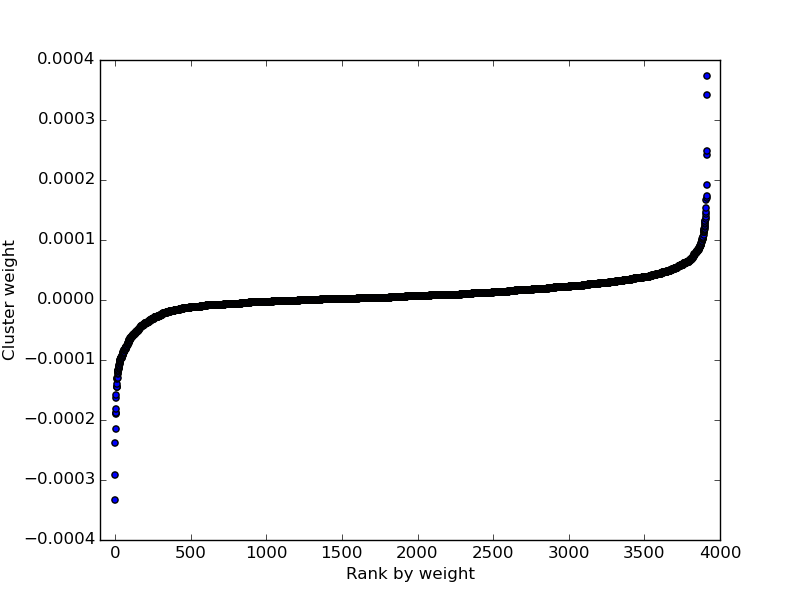
\includegraphics[scale=0.4]{./instance-scatter.png}
\caption{This diagram illustrates the distribution of the instance weights assigned by CAMIL H-BoW. The Y-Axis shows the weights, while the X-Axis shows the ranking of the clusters by weight. Clearly, there are a relatively small number of clusters that have disproportionately large weights or small weights, while the vast majority of the 3918 clusters have weights close to 0.} \label{instance-scatter}
\end{figure}

In the original MGWAS paper, the authors identify 50 important gene markers with mRMR that are used for their classifier. Conversely, CAMIL uses all of the data to train and test the classifier, resulting in 3918 clusters, and subsequently identifies significant clusters based on the classification results. Figure \ref{instance-scatter} is a visual display of the cluster weights determined by CAMIL, using the 344 patient training set and 23 patient test set. Clearly, there are a few clusters with disproportionately high or low weights, while most clusters have weights near 0. Concretely, the lowest cluster weight is -0.000333, the highest is 0.000374, the mean is 0.000008, and the median is 0.000006. Intuitively, this appears to make sense, as there should be a relatively small number of key clusters whose presence is actually indicative of type 2 diabetes, while most other clusters are not particularly relevant in this case and whose weights are just noise. Thus, the weights obtained by this method appear to be plausible. In contrast, the labels obtained by GICF were barely differentiated from each other at all.
